
\documentclass[12pt,letterpaper,fleqn]{hmcpset}
\usepackage[margin=1in]{geometry}
\usepackage{graphicx}
\usepackage{amsmath,amssymb}
\usepackage{enumerate}
\usepackage{hyperref}
\usepackage{parskip}
\usepackage{listings}

\DeclareMathOperator\erf{erf}

% Theorems
\usepackage{amsthm}
\renewcommand\qedsymbol{$\blacksquare$}
\makeatletter
\@ifclassloaded{article}{
    \newtheorem{definition}{Definition}[section]
    \newtheorem{example}{Example}[section]
    \newtheorem{theorem}{Theorem}[section]
    \newtheorem{corollary}{Corollary}[theorem]
    \newtheorem{lemma}{Lemma}[theorem]
}{
}
\makeatother

% Random Stuff
\setlength\unitlength{1mm}

\newcommand{\insertfig}[3]{
\begin{figure}[htbp]\begin{center}\begin{picture}(120,90)
\put(0,-5){\includegraphics[width=12cm,height=9cm,clip=]{#1.eps}}\end{picture}\end{center}
\caption{#2}\label{#3}\end{figure}}

\newcommand{\insertxfig}[4]{
\begin{figure}[htbp]
\begin{center}
\leavevmode \centerline{\resizebox{#4\textwidth}{!}{\input
#1.pstex_t}}
\caption{#2} \label{#3}
\end{center}
\end{figure}}

\long\def\comment#1{}

\newcommand\norm[1]{\left\lVert#1\right\rVert}
\DeclareMathOperator*{\argmin}{arg\,min}
\DeclareMathOperator*{\argmax}{arg\,max}

% bb font symbols
\newfont{\bbb}{msbm10 scaled 700}
\newcommand{\CCC}{\mbox{\bbb C}}

\newfont{\bbf}{msbm10 scaled 1100}
\newcommand{\CC}{\mbox{\bbf C}}
\newcommand{\PP}{\mbox{\bbf P}}
\newcommand{\RR}{\mbox{\bbf R}}
\newcommand{\QQ}{\mbox{\bbf Q}}
\newcommand{\ZZ}{\mbox{\bbf Z}}
\renewcommand{\SS}{\mbox{\bbf S}}
\newcommand{\FF}{\mbox{\bbf F}}
\newcommand{\GG}{\mbox{\bbf G}}
\newcommand{\EE}{\mbox{\bbf E}}
\newcommand{\NN}{\mbox{\bbf N}}
\newcommand{\KK}{\mbox{\bbf K}}
\newcommand{\KL}{\mbox{\bbf KL}}

% Vectors
\renewcommand{\aa}{{\bf a}}
\newcommand{\bb}{{\bf b}}
\newcommand{\cc}{{\bf c}}
\newcommand{\dd}{{\bf d}}
\newcommand{\ee}{{\bf e}}
\newcommand{\ff}{{\bf f}}
\renewcommand{\gg}{{\bf g}}
\newcommand{\hh}{{\bf h}}
\newcommand{\ii}{{\bf i}}
\newcommand{\jj}{{\bf j}}
\newcommand{\kk}{{\bf k}}
\renewcommand{\ll}{{\bf l}}
\newcommand{\mm}{{\bf m}}
\newcommand{\nn}{{\bf n}}
\newcommand{\oo}{{\bf o}}
\newcommand{\pp}{{\bf p}}
\newcommand{\qq}{{\bf q}}
\newcommand{\rr}{{\bf r}}
\renewcommand{\ss}{{\bf s}}
\renewcommand{\tt}{{\bf t}}
\newcommand{\uu}{{\bf u}}
\newcommand{\ww}{{\bf w}}
\newcommand{\vv}{{\bf v}}
\newcommand{\xx}{{\bf x}}
\newcommand{\yy}{{\bf y}}
\newcommand{\zz}{{\bf z}}
\newcommand{\0}{{\bf 0}}
\newcommand{\1}{{\bf 1}}

% Matrices
\newcommand{\Ab}{{\bf A}}
\newcommand{\Bb}{{\bf B}}
\newcommand{\Cb}{{\bf C}}
\newcommand{\Db}{{\bf D}}
\newcommand{\Eb}{{\bf E}}
\newcommand{\Fb}{{\bf F}}
\newcommand{\Gb}{{\bf G}}
\newcommand{\Hb}{{\bf H}}
\newcommand{\Ib}{{\bf I}}
\newcommand{\Jb}{{\bf J}}
\newcommand{\Kb}{{\bf K}}
\newcommand{\Lb}{{\bf L}}
\newcommand{\Mb}{{\bf M}}
\newcommand{\Nb}{{\bf N}}
\newcommand{\Ob}{{\bf O}}
\newcommand{\Pb}{{\bf P}}
\newcommand{\Qb}{{\bf Q}}
\newcommand{\Rb}{{\bf R}}
\newcommand{\Sb}{{\bf S}}
\newcommand{\Tb}{{\bf T}}
\newcommand{\Ub}{{\bf U}}
\newcommand{\Wb}{{\bf W}}
\newcommand{\Vb}{{\bf V}}
\newcommand{\Xb}{{\bf X}}
\newcommand{\Yb}{{\bf Y}}
\newcommand{\Zb}{{\bf Z}}

% Calligraphic
\newcommand{\Ac}{{\cal A}}
\newcommand{\Bc}{{\cal B}}
\newcommand{\Cc}{{\cal C}}
\newcommand{\Dc}{{\cal D}}
\newcommand{\Ec}{{\cal E}}
\newcommand{\Fc}{{\cal F}}
\newcommand{\Gc}{{\cal G}}
\newcommand{\Hc}{{\cal H}}
\newcommand{\Ic}{{\cal I}}
\newcommand{\Jc}{{\cal J}}
\newcommand{\Kc}{{\cal K}}
\newcommand{\Lc}{{\cal L}}
\newcommand{\Mc}{{\cal M}}
\newcommand{\Nc}{{\cal N}}
\newcommand{\Oc}{{\cal O}}
\newcommand{\Pc}{{\cal P}}
\newcommand{\Qc}{{\cal Q}}
\newcommand{\Rc}{{\cal R}}
\newcommand{\Sc}{{\cal S}}
\newcommand{\Tc}{{\cal T}}
\newcommand{\Uc}{{\cal U}}
\newcommand{\Wc}{{\cal W}}
\newcommand{\Vc}{{\cal V}}
\newcommand{\Xc}{{\cal X}}
\newcommand{\Yc}{{\cal Y}}
\newcommand{\Zc}{{\cal Z}}

% Bold greek letters
\newcommand{\alphab}{\hbox{\boldmath$\alpha$}}
\newcommand{\betab}{\hbox{\boldmath$\beta$}}
\newcommand{\gammab}{\hbox{\boldmath$\gamma$}}
\newcommand{\deltab}{\hbox{\boldmath$\delta$}}
\newcommand{\etab}{\hbox{\boldmath$\eta$}}
\newcommand{\lambdab}{\hbox{\boldmath$\lambda$}}
\newcommand{\epsilonb}{\hbox{\boldmath$\epsilon$}}
\newcommand{\nub}{\hbox{\boldmath$\nu$}}
\newcommand{\mub}{\hbox{\boldmath$\mu$}}
\newcommand{\zetab}{\hbox{\boldmath$\zeta$}}
\newcommand{\phib}{\hbox{\boldmath$\phi$}}
\newcommand{\psib}{\hbox{\boldmath$\psi$}}
\newcommand{\thetab}{\hbox{\boldmath$\theta$}}
\newcommand{\taub}{\hbox{\boldmath$\tau$}}
\newcommand{\omegab}{\hbox{\boldmath$\omega$}}
\newcommand{\xib}{\hbox{\boldmath$\xi$}}
\newcommand{\sigmab}{\hbox{\boldmath$\sigma$}}
\newcommand{\pib}{\hbox{\boldmath$\pi$}}
\newcommand{\rhob}{\hbox{\boldmath$\rho$}}

\newcommand{\Gammab}{\hbox{\boldmath$\Gamma$}}
\newcommand{\Lambdab}{\hbox{\boldmath$\Lambda$}}
\newcommand{\Deltab}{\hbox{\boldmath$\Delta$}}
\newcommand{\Sigmab}{\hbox{\boldmath$\Sigma$}}
\newcommand{\Phib}{\hbox{\boldmath$\Phi$}}
\newcommand{\Pib}{\hbox{\boldmath$\Pi$}}
\newcommand{\Psib}{\hbox{\boldmath$\Psi$}}
\newcommand{\Thetab}{\hbox{\boldmath$\Theta$}}
\newcommand{\Omegab}{\hbox{\boldmath$\Omega$}}
\newcommand{\Xib}{\hbox{\boldmath$\Xi$}}

% mixed symbols
\newcommand{\sinc}{{\hbox{sinc}}}
\newcommand{\diag}{{\hbox{diag}}}
\renewcommand{\det}{{\hbox{det}}}
\newcommand{\trace}{{\hbox{tr}}}
\newcommand{\tr}{\trace}
\newcommand{\sign}{{\hbox{sign}}}
\renewcommand{\arg}{{\hbox{arg}}}
\newcommand{\var}{{\hbox{var}}}
\newcommand{\cov}{{\hbox{cov}}}
\renewcommand{\Re}{{\rm Re}}
\renewcommand{\Im}{{\rm Im}}
\newcommand{\eqdef}{\stackrel{\Delta}{=}}
\newcommand{\defines}{{\,\,\stackrel{\scriptscriptstyle \bigtriangleup}{=}\,\,}}
\newcommand{\<}{\left\langle}
\renewcommand{\>}{\right\rangle}
\newcommand{\Psf}{{\sf P}}
\newcommand{\T}{\top}
\newcommand{\m}[1]{\begin{bmatrix} #1 \end{bmatrix}}

% info for header block in upper right hand corner
\name{Nathaniel Diamant}
\class{Math 189r}
\assignment{Homework 1}
\duedate{September 19, 2016}

\begin{document}

There are 8 problems in this set. 4 of the problems (you choose except this first
set must include problem 1 and/or 2) are due on September 12,
and the rest of the problems are due on September 19. Feel
free to work with other students, but make sure you write up the homework
and code on your own (no copying homework \textit{or} code; no pair programming).
Feel free to ask students or instructors for help debugging code or whatever else,
though.
When implementing algorithms you may not use any library (such as \texttt{sklearn})
that already implements the algorithms but you may use any other library for
data cleaning and numeric purposes (\texttt{numpy} or \texttt{pandas}). Use common
sense. Problems are in no specific order.\\[1em]


\textbf{1} (\textbf{regression}). Download the data at 
\url{https://math189r.github.io/hw/data/online_news_popularity/online_news_popularity.csv}
and the info file at
\url{https://math189r.github.io/hw/data/online_news_popularity/online_news_popularity.txt}.
Read the info file. Split the csv file into a training and test set with
the first two thirds of the data in the training set and the rest for testing.
Of the testing data, split the first half into a `validation set' (used
to optimize hyperparameters while leaving your testing data pristine) and
the remaining half as your test set.
We will use this data for the remainder of the problem. The goal of this data
is to predict the \textbf{log} number of shares a news article will have given the other
features.
\begin{enumerate}[(a)]
    \item (\textbf{math}) Show that the maximum a posteriori problem for
        linear regression with a zero-mean Gaussian prior $\PP(\ww) = \prod_j
        \Nc(w_j | 0, \tau^2)$ on the weights,
        \[
            \argmax_\ww \sum_{i=1}^N \log\Nc(y_i | w_0 + \ww^\T\xx_i, \sigma^2) + \sum_{j=1}^D \log\Nc(w_j | 0, \tau^2)
        \]
        is equivalent to the ridge regression problem
        \[
            \argmin \frac{1}{N}\sum_{i=1}^N (y_i - (w_0 + \ww^\T\xx_i))^2 + \lambda ||\ww||_2^2
        \]
    \item (\textbf{math}) Find a closed form solution $\xx^\star$ to the ridge regression
        problem:
        \[
            \text{minimize: } ||A\xx - \bb||_2^2 + ||\Gamma\xx||_2^2.
        \]
    \item (\textbf{implementation}) Attempt to predict the $\log\text{shares}$ using ridge
        regression from the previous problem solution. Make sure you include a bias
        term and \textit{don't regularize the bias term}.
        Find the optimal regularization parameter $\lambda$
        from the validation set. Plot both $\lambda$ versus the validation RMSE (you should have
        tried at least 150 parameter settings randomly chosen between 0.0 and 150.0 because
        the dataset is small)
        and $\lambda$ versus $||\thetab^\star||_2$ where $\thetab$ is your weight vector.
        What is the final RMSE on the test set with the optimal $\lambda^\star$?
    \item (\textbf{math}) Consider regularized linear regression where we pull the
        basis term out of the feature vectors. That is, instead of computing $\hat\yy
        = \thetab^\T\xx$ with $\xx_0 = 1$, we compute $\hat\yy = \thetab^\T\xx + b$.
        This corresponds to solving the optimization problem
        \[
            \text{minimize: } ||A\xx + b\1 - \yy||_2^2 + ||\Gamma\xx||_2^2.
        \]
        Solve for the optimal $\xx^\star$ explicitly. Use this close form to compute the
        bias term for the previous problem (with the same regularization strategy). Make
        sure it is the same.
    \item (\textbf{implementation}) We can also compute the solution to the least squares
        problem using gradient descent. Consider the same bias-relocated objective
        \[
            \text{minimize: } f = ||A\xx + b\1 - \yy||_2^2 + ||\Gamma\xx||_2^2.
        \]
        Compute the gradients and run gradient descent. Plot the $\ell_2$ norm
        between the optimal $(\xx^\star, b^\star)$ vector you computed in closed form
        and the iterates generated by gradient descent. Hint: your plot should move
        down and to the left and approach zero as the number of iterations increases. If
        it doesn't, try decreasing the learning rate.
\end{enumerate}

\vspace{15mm}

\begin{enumerate}[(a)]
    \item 
        We will begin by taking the log of $\Nc$.
            \begin{align*}
               \log(\Nc(x|\mu,\sigma^2)) &= \log\left(\frac{1}{\sqrt{2\pi\sigma^2}}\exp\left(-\frac{(x-\mu)^2}{2\sigma^2}\right)\right)\\
               &=-\frac{(x-\mu)^2}{2\sigma^2} \log\left( \frac{1}{\sqrt{2\pi\sigma^2}} \right)\\
               &= \frac{(x-\mu)^2}{2\sigma^2} - \log \left( \sqrt{2 \pi }\sigma \right)
            \end{align*}
            
            So our problem becomes,
                
                $$\argmax_\ww \sum_{i=1}^N \log\Nc(y_i | w_0 + \ww^\T\xx_i, \sigma^2) + \sum_{j=1}^D \log\Nc(w_j | 0, \tau^2) - N\log \left( \sqrt{2 \pi }\sigma \right) - D\log \left( \sqrt{2 \pi }\tau \right) $$ \\
                $$\argmax_\ww -\frac{1}{2\sigma^2}\sum_{i=1}^N (y_i-(w_0 + \ww^\T \xx_i))^2 - \frac{1}{2 \tau^2 } \sum_{j=1}^D (\omega_j)^2$$
            
            We can factor out the $1/2$, multiply by $\sigma^2$ and $\sum_{j=1}^D (\omega_j)^2 = \ww \ww^\T = ||\ww||_2^2$ and maximizing the negative is the same as minimizing the positive, so we get,
                $$  \argmin_\ww \sum_{i=1}^N (y_i-(w_0 + \ww^\T\xx_i))^2 + \frac{\sigma^2}{\tau^2} ||\ww||_2^2$$
            Now we substitute $\lambda = \frac{\sigma^2}{\tau^2}$,
                \[
                \argmin \sum_{i=1}^N (y_i - (w_0 + \ww^\T\xx_i))^2 + \lambda||\ww||_2^2
                \]
            as desired.
    \item
        To solve the following problem, we will take the gradient with respect to $\xx$ and set it to zero,
            $$\text{minimize: } ||A\xx - \bb||_2^2 + ||\Gamma\xx||_2^2$$
        We will begin by expanding the norms.
            \begin{align*}
                ||A\xx - \bb||_2^2 + ||\Gamma\xx||_2^2 &= (A\xx - \bb)^\T(A\xx - \bb) + (\Gamma \xx)^\T \Gamma \xx \\
                &= \xx^\T A^\T A \xx - \xx^\T A^\T \bb - \bb^\T A \xx + \xx^\T \Gamma^\T \Gamma \xx \\ 
            \end{align*}
        Now we take the gradient with respect to $\xx$ and set to zero,
            \begin{align*}
                \nabla_\xx \left[ \xx^\T A^\T A \xx - \xx^\T A^\T \bb - \bb^\T A \xx + \xx^\T \Gamma^\T \Gamma \xx  \right]&= 0\\
                 \nabla_\xx \tr \left[ \xx^\T A^\T A \xx - \xx^\T A^\T \bb - \bb^\T A \xx + \xx^\T \Gamma^\T \Gamma \xx  \right] &= 0 \text{   Using trace of scalar $a$ equals $a$} \\
                 \nabla_\xx \left[ \tr \xx^\T A^\T A \xx - 2\tr \xx^\T A^\T \bb + \tr \xx^\T \Gamma^\T \Gamma \xx  \right] &= 0 \text{   Using $\tr A = \tr A^\T$}\\
                 2A^\T A \xx -2A^\T \bb + 2\Gamma^\T \Gamma \xx &= 0\\
                 \left( A^\T A + \Gamma^\T \Gamma \right) \xx &= A^\T\bb \\
                 \xx &= \left( A^\T A + \Gamma^\T \Gamma \right)^{-1} A^\T \bb
            \end{align*}
        Which is our closed form solution for $\xx$.
    \item
        \lstinputlisting[language=Python]{Ridge+Closed+Form.py}
        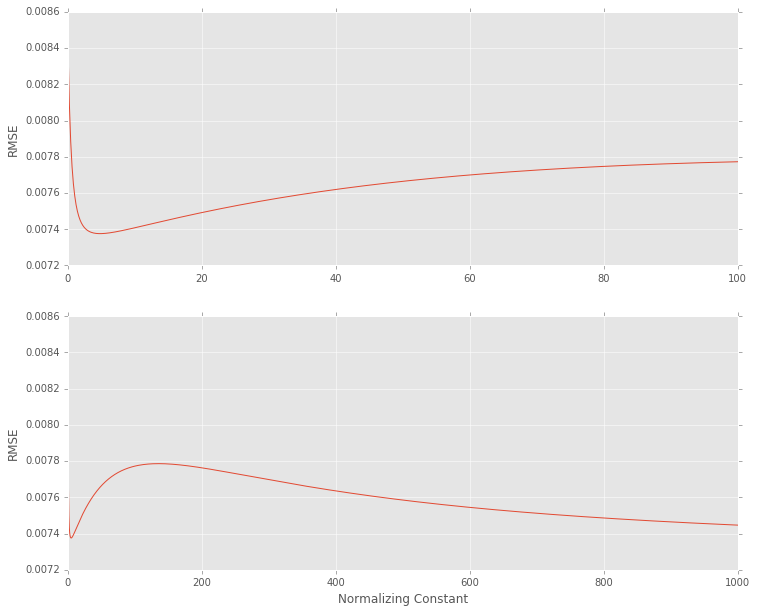
\includegraphics[scale = .5]{RMSEvNormconst.png}\\
        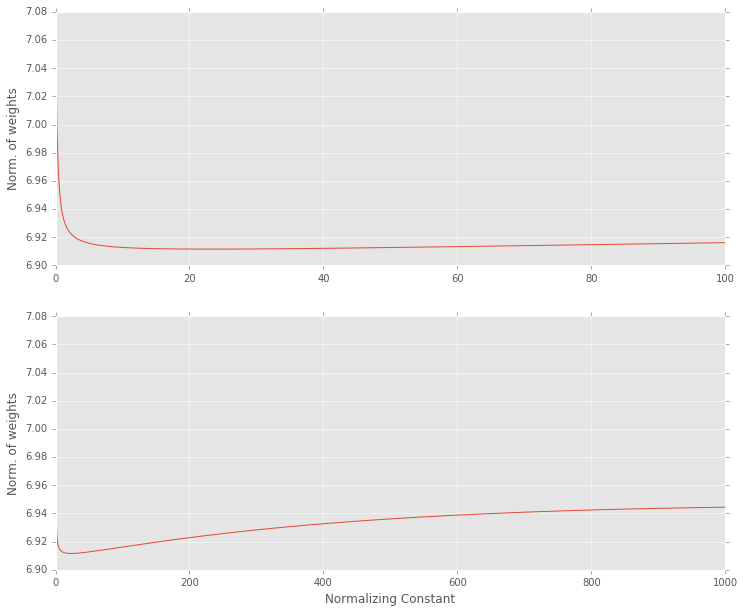
\includegraphics[scale = .5]{wNormVNormconst.png}
    \item
        We will begin by distributing the norm.
        \begin{align*}
            ||A\xx + b\1 -\yy||_2^2 + ||\Gamma\xx||_2^2 &= (A\xx + b\1 -\yy)^\T(A\xx + b\1 -\yy) + (\Gamma \xx)^\T \Gamma \xx\\
            &= \xx^\T A^\T A \xx + 2 \xx^\T A^\T b\1 - 2 \xx^\T A^\T \yy -2 \yy^\T b\1 + b\1^\T b\1 \\ &\qquad + \yy^T \yy + \xx^\T \Gamma^\T \Gamma \xx
        \end{align*}
        Now we take the gradient and set to zero.
        \begin{align*}
            \nabla_\xx \left[ \xx^\T A^\T A \xx + 2 \xx^\T A^\T b\1 - 2 \xx^\T A^\T \yy -2 \yy^\T b\1 + b\1^\T b\1 + \yy^T \yy + \xx^\T \Gamma^\T \Gamma \xx \right] &= 0\\
            2A^\T A \xx + 2 A^\T b\1 - 2 A^\T \yy + 2\Gamma^\T \Gamma \xx &= 0 \\
            (A^\T A + \Gamma^\T \Gamma)\xx &= A^\T (\yy  - b\1) \\
            (A^\T A + \Gamma^\T \Gamma)^{-1}A^\T (\yy  - b\1) &= \xx
        \end{align*}
        Which gives our closed form. Now to solve for the bias terms we will take the derivative with respect to $b$ and set to zero.
        \begin{align*}
            \frac{d}{db} \left[  \xx^\T A^\T A \xx + 2 \xx^\T A^\T b\1 - 2 \xx^\T A^\T \yy -2 \yy^\T b\1 + b\1^\T b\1 + \yy^T \yy + \xx^\T \Gamma^\T \Gamma \xx \right] &= 0\\
            2 \xx^\T A^\T\1 -2\yy^\T\1 +2 b N &= 0 \\
             \frac{\yy^\T\1 - \xx^\T A^\T\1}{N} &= b
        \end{align*}
        Where $N$ is the number of training points. Now we have a system of two equations. If we substitute the solution for $b$ into the solution for $\xx$, then we get the solution for $x$, which we could plug back into the solution for $b$ to get our answer. To do so, we will use the fact that, because it is a scalar, $\xx^\T A^\T\1 = \1^\T A \xx$
        \begin{align*}
            2A^\T A \xx + 2 A^\T b\1 - 2 A^\T \yy + 2\Gamma^\T \Gamma \xx &= 0 \\
            (A^\T A + \Gamma^\T \Gamma)\xx + \frac{\1^\T \yy - \1^\T A \xx}{N}A^\T \1 - A^\T \yy  &= 0\\
            \xx =  \left(A^\T A + \Gamma^\T \Gamma -\frac{A^\T\1\1^\T A}{N}\right)^{-1} \left(A^\T \yy - \frac{A^\T \1 \1^T \yy}{N} \right)
        \end{align*}

    \item
        As we saw in part (d), the gradient with respect to $\xx$ is
            $$ (A^\T A + \Gamma^\T \Gamma)\xx - A^\T (\yy  - b\1)$$
        And the derivative with respect to $b$ is 
            $$\xx^\T A^\T\1 -\yy^\T\1 +2 b N$$
        So we will randomly initialize the weights for $\xx$ and $b$ normally with mean $0$ and then subtract the gradient and derivative respectively each step. The code:
        \lstinputlisting[language=Python]{Ridge+Regression+Gradient+Descent.py}
        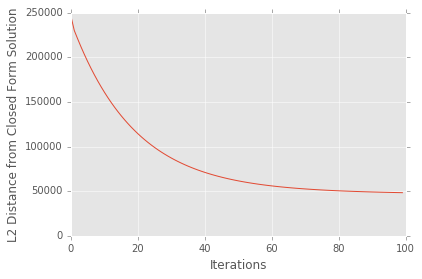
\includegraphics[scale = .8]{graddescent.png}


\end{enumerate}


\newpage

\textbf{2} (\textbf{MNIST}) Download the training set at 
\url{http://pjreddie.com/media/files/mnist_train.csv} and test set at
\url{http://pjreddie.com/media/files/mnist_test.csv}. This dataset, the MNIST
dataset, is a classic in the deep learning literature as a toy dataset to test
algorithms on. The problem is this: we have $28\times 28$ images of handwritten
digits as well as the label of which digit $0 \leq \texttt{label} \leq 9$ the written
digit corresponds to. Given a new image of a handwritten digit, we want to be
able to predict which digit it is.
The format of the data is \texttt{label, pix-11, pix-12, pix-13, ...}
where \texttt{pix-ij} is the pixel in the \texttt{ith} row and \texttt{jth} column.
\begin{enumerate}[(a)]
    \item (\textbf{logistic}) Restrict the dataset to only the digits with a label
        of 0 or 1. Implement L2 regularized logistic regression as a model to compute
        $\PP(y=1|\xx)$ for a different value of the regularization parameter $\lambda$.
        Plot the learning curve (objective vs. iteration) when using Newton's Method
        \textit{and} gradient descent.
        Plot the accuracy, precision ($p = \PP(y=1 | \hat y=1)$), recall ($r = \PP(\hat y=1 | y=1)$),
        and F1-score ($F1 = 2pr / (p+r)$) for different values of $\lambda$ (try at least
        10 different values including $\lambda = 0$) on the test set and report the
        value of $\lambda$ which maximizes the accuracy on the test set. What is your
        accuracy on the test set for this model? Your accuracy should definitely be
        over 90\%.

    \item (\textbf{softmax}) Now we will use the whole dataset and predict the label
        of each digit using L2 regularized softmax regression (multinomial logistic
        regression). Implement this using gradient descent, and plot the accuracy
        on the test set for different values of $\lambda$, the regularization parameter.
        Report the test accuracy for the optimal value of $\lambda$ as well as it's
        learning curve. Your accuracy should be over 90\%.

    \item (\textbf{KNN}) Solve the same problem posed in part (b) but use
        K-Nearest Neighbors instead of softmax regression and vary $k$ instead
        of $\lambda$. Only try 3 values for $k$ ($1,5,$ and $10$) and the $\ell_2$
        norm as your metric. Plot and report the same results as part (b).
\end{enumerate}

\newpage

\textbf{3} (\textbf{Murphy 2.11} and \textbf{2.16})
\begin{enumerate}[(a)]
    \item Derive the normalization constant ($Z$) for a one dimensional
        zero-mean Gaussian
        \[
            \PP(x; \sigma^2) = \frac{1}{Z}\exp\left(-\frac{x^2}{2\sigma^2}\right)
        \]
        such that $\PP(x; \sigma^2)$ becomes a valid density.
    \item Suppose $\theta \sim \text{Beta}(a,b)$ such
        that
        \[
            \PP(\theta; a,b) = \frac{1}{B(a,b)} \theta^{a-1}(1-\theta)^{b-1} = \frac{\Gamma(a+b)}{\Gamma(a)\Gamma(b)} \theta^{a-1}(1-\theta)^{b-1}
        \]
        where $B(a,b) = \Gamma(a)\Gamma(b)/\Gamma(a+b)$ is the Beta function
        and $\Gamma(x)$ is the Gamma function.
        Derive the mean, mode, and variance of $\theta$.
\end{enumerate}

\begin{solution}
	(a) We have to find $Z$ such that
	$$\int_{-\infty}^{\infty}\frac{1}{Z}\exp\left(-\frac{x^2}{2\sigma^2}\right)dx = 1$$
	This means that
	$$\int_{-\infty}^{\infty}\exp\left(-\frac{x^2}{2\sigma^2}\right)dx = Z$$
	and that, 
	$$ Z^2 = \int_{-\infty}^{\infty}\exp\left(-\frac{x^2}{2\sigma^2}\right)dx \cdot \int_{-\infty}^{\infty}\exp\left(-\frac{y^2}{2\sigma^2}\right)dy $$
	Now we combine the integrals into,
	$$ = \int_{-\infty}^{\infty}\int_{-\infty}^{\infty}\exp\left(-\frac{x^2+y^2}{2\sigma^2}\right)dxdy $$
	That $x^2 + y^2$ looks familiar. If we convert to polar coordinates, we get:
	$$ = \int_{0}^{2\pi}\int_{0}^{\infty}\exp\left(-\frac{r^2}{2\sigma^2}\right)rdrd\theta $$
	Now we can use a u-substition, $u=r^2/(2\sigma^2)$, $du = r/\sigma^2dr$. This yields,
	$$Z^2 = -2\pi \sigma^2 \left[ e^{-u} \right]_0^\infty$$
	So $\fbox{$Z=\sigma\sqrt{2\pi}$}$\\

    (b) The mean is calculated by integrating over the support of the distribution,
        \begin{align*}
            \EE(\theta) &= \frac{1}{B(a,b)} \int_{\SS} \theta \theta^{a-1}(1-\theta)^{b-1} d\theta \\
            &=  \frac{1}{B(a,b)} \int_{0}^1 \theta^{a}(1-\theta)^{b-1} d\theta
        \end{align*}
    But $\frac{1}{B(a,b)}$ normalizes $\int_{\SS} \theta^{a-1}(1-\theta)^{b-1} d\theta$, so $\frac{1}{B(a+1,b)}$ normalizes $\int_{0}^1 \theta^{a}(1-\theta)^{b-1} d\theta$. So,
        \begin{align*}
            \EE(\theta) &= \frac{1}{B(a,b)} B(a+1,b) \\
            &= \frac{\Gamma(a+b)}{\Gamma(a)\Gamma(b)} \frac{\Gamma(a+1)\Gamma(b)}{\Gamma(a + b +1)}\\
            &= a\frac{\Gamma(a+b)}{\Gamma(a)\Gamma(b)} \frac{\Gamma(a)\Gamma(b)}{(a+b)\Gamma(a + b)}\\
            &= \frac{a}{a+b}
        \end{align*}
        Now we find the variance. 
        \begin{align*}
            \sigma^2 &= \EE(\theta^2) - \EE(\theta)^2 \\
            &= \frac{1}{B(a,b)} \int_{0}^1 \theta^2 \theta^{a - 1}(1-\theta)^{b-1} d\theta - \EE(\theta)^2\\
            &= \frac{1}{B(a,b)} B(a+2,b) - \EE(\theta)^2 \\
            &= \frac{\Gamma(a+b)}{\Gamma(a)\Gamma(b)} \frac{\Gamma(a+2)\Gamma(b)}{\Gamma(a + b + 2)} - \EE(\theta)^2 \\
            &= \frac{\Gamma(a+b)}{\Gamma(a)\Gamma(b)} \frac{(a+1)(a)\Gamma(a)\Gamma(b)}{(a + b +1)(a+b)\Gamma(a + b)} - \EE(\theta)^2\\
            &= \frac{a(a+1)}{(a+b+1)(a+b)} - \frac{a^2}{(a+b)^2}\\
            &= \frac{a(a+1)(a+b)-(a+b+1)a^2}{(a+b)^2(a+b+1)}\\
            &= \frac{a b}{(a+b)^2 (a+b+1)} \text{  Thanks Mathematica}
        \end{align*}
        Now we find the mode. To find the mode, we set the derivative to zero.
            \begin{align*}
                \frac{d}{d \theta} \frac{1}{B(a,b)} \theta^{a-1}(1-\theta)^{b-1} &= 0\\
                (a-1)\theta^{a-2}(1-\theta)^{b-1} - (b-1)\theta^{a-1}(1-\theta)^{b-2}&=0\\   
            \end{align*}
        We will ignore the $\theta = 0,1$ solutions, because they represent minima of the distribution. 
            \begin{align*}
                ((1-\theta)(a-1) + \theta(b-1))\theta^{a-2}\theta^{b-2} &= 0\\
                ((1-\theta)(a-1) + \theta(b-1)) &= 0\\
                \theta &= \frac{a-1}{a+b-2} \text{ Thanks again, Mathematica}
            \end{align*}
    \end{solution}

\newpage




\textbf{4} (\textbf{Murphy 2.15}) Let $\PP_{emp}(x)$ be the empirical distribution and let
$q(x|\thetab)$ be some model. Show that $\argmin_q \KL(\PP_{emp} || q)$ is obtained by
$q(x) = q(x ; \hat\thetab)$ where $\hat\thetab = \argmax_{\thetab} \;\Lc(q, \Dc)$ is
the maximum likelihood estimate.

\vspace{15mm}
We begin with definition of $\KL$ divergence.
\begin{align*}
    \KL(\PP_{emp} || q) &= \int_{-\infty}^{\infty}\PP_{emp}(x)\log \left(\frac{\PP_{emp}(x)}{q(x)} \right)dx\\
    &= \int_{-\infty}^{\infty}\PP_{emp}(x)\log(\PP_{emp}(x))dx - \int_{-\infty}^{\infty}\PP_{emp}(x)\log(q(x))dx\\
\end{align*}
We have no control over the first term, so for the purpose of our minimization problem it becomes a constant. Constants do not change optimization problems. Then all we are left with is the second term. If we expand using the defininition of the empirical distribution, we get,

    $$- \int_{-\infty}^{\infty}\PP_{emp}(x)\log(q(x))dx = -\frac{1}{N}\sum_{i=1}^{N}\delta_{x_i}(A)log(q(A))$$

Where $N$ is the number of data points. We are trying to minimize a negative value, which is equivalent to maximizing the positive of the same value. We also know that $\frac{1}{N}$ is a positive constant. That means that if we take $\exp(\sum_{i=1}^{N}\delta_{x_i}(A)log(q(A)))$, it will be an equivalent maximization problem. This yields,
\begin{align*}
    exp(\frac{1}{N}\sum_{i=1}^{N}\delta_{x_i}(A)log(q(A))) &= \prod_{i=1}^N \exp(\delta_i(A))\exp(\log(q(A))\\
    &= \prod_{i=1}^N \exp(\delta_i(A)) \prod_{i=1}^N q(A)
\end{align*}
Again, $\prod_{i=1}^N \exp(\delta_i(A))$ is a positive constant, so we can ignore it in our maximization. That leaves only the product of $q(A)$ to maximize. But $\prod_{i=1}^N q(A) = \Lc(q,\Dc)$, so we have shown that maximizing the likelihood is equivalent to minimizing the KL divergence between the empirical distribution and our model.

\newpage

\textbf{5} (\textbf{Linear Transformation}) Let $\yy = A\xx + \bb$ be a random vector.
show that expectation is linear:
\[
    \EE[\yy] = \EE[A\xx + \bb] = A\EE[\xx] + \bb.
\]
Also show that
\[
    \cov[\yy] = \cov[A\xx + \bb] = A \cov[\xx] A^\T = A\Sigmab A^\T.
\]

\vspace{10mm}

Let $p$ with support $\SS$ be the distribution $\xx$ is drawn from. Then
	$$\EE[\yy] = \int_{\SS} y(\xx) p(\xx)dx = \int_{\SS} (A\xx + \bb) p(\xx)dx$$
We can distribute the $p(\xx)dx$ and split into two integrals:
	$$\int_{\SS} A\xx p(\xx)dx + \int_{\SS} \bb p(\xx)dx$$
Both $A$ and $\bb$ are constant, which leaves:
	$$A \int_{\SS} \xx p(\xx)dx + \bb \int_{\SS}  p(\xx)dx$$
The first term is just the expected value of $\xx$ and the second integral by definition of a probability distribution evaluates to 1. That leaves,
	$$A\EE[\xx] + \bb$$
As desired.\\\\

Now to find the covariance. The covariance matrix,
    $$\cov(\yy) = \EE[(\yy - \EE(\yy)(\yy - \EE(\yy)^\T]$$. 
We can calculate $\yy - \EE(\yy)$ from the previous part.
    $$(\yy - \EE(\yy) = A\xx + \bb - (A\EE[\xx] + \bb) = A(\xx - \EE[\xx])$$
Now we can find $cov(\yy)$,
    $$cov(\yy) = \EE[A(\xx - \EE[\xx])(A(\xx - \EE[\xx]))^\T] = \EE[A(\xx - \EE[\xx])(\xx - \EE[\xx])^\T A^\T]$$
The middle two terms are the covariance matrix of $\xx$, so
    $$cov(\yy) = \EE[A\Sigmab_\xx A^\T] = A\Sigmab_\xx A^\T$$
As desired.


\newpage



\textbf{6} Given the dataset $\Dc = \{(x,y)\} = \{(0,1), (2,3), (3,6), (4,8)\}$
\begin{enumerate}[(a)]
    \item Find the least squares estimate $y = \thetab^\T\xx$ by hand using
        Cramer's Rule.
    \item Use the normal equations to find the same solution and verify it
        is the same as part (a).
    \item Plot the data and the optimal linear fit you found.
    \item Find randomly generate 100 points near the line with white Gaussian
        noise and then compute the least squares estimate (using a computer).
        Verify that this new line is close to the original and plot the new
        dataset, the old line, and the new line.
\end{enumerate}

\vspace{15mm}

\begin{enumerate}[(a)]
    \item 
        The closed form solution can be found using the closed form:
        \begin{align*}
            (A^\T A)\thetab &= A^\T \yy \\
            \left(
                \begin{bmatrix} 
                1 & 1 & 1 & 1\\
                0 & 2 & 3 & 4          
                \end{bmatrix}
                \begin{bmatrix} 
                1 & 0 \\
                1 & 2 \\
                1 & 3 \\
                1 & 4\\          
                \end{bmatrix}              
                \right)\thetab
                &= 
                \begin{bmatrix} 
                1 & 1 & 1 & 1\\
                0 & 2 & 3 & 4          
                \end{bmatrix} 
                \begin{bmatrix}
                1 \\
                3 \\
                6 \\
                8 \\ 
                \end{bmatrix}\\
                \begin{bmatrix}
                 4 & 9 \\
                 9 & 29 \\
                \end{bmatrix} \thetab
                &= 
                \begin{bmatrix}
                 18 \\
                 56 \\
                \end{bmatrix}\\
        \end{align*}
        Now we use Cramer's rule. First, 
        $$\begin{vmatrix}
                 4 & 9 \\
                 9 & 29 \\
            \end{vmatrix} = 35 = D$$.
        \begin{align*}
            \theta_1 &= \frac{
                \begin{vmatrix}
                    18 & 9\
                    56 & 29
                \end{vmatrix}
            }{D} = 18/35\\
            \theta_2 &= \frac{
                \begin{vmatrix}
                    4 & 18\
                    9 & 56
                \end{vmatrix}
            }{D} =62/35
        \end{align*}
         
    \item
        Now we use $\thetab = (A^\T A)^{-1}A^\T \yy$. Mathematica gives 
        $\theta = \left(
\begin{array}{c}
 \frac{18}{35} \\
 \frac{62}{35} \\
\end{array}
\right)$.

    \item

         
\end{enumerate}
\newpage

\textbf{7} (\textbf{Murphy 8.3}) Gradient and Hessian of the log-likelihood for
logistic regression.
\begin{enumerate}[(a)]
    \item Let $\sigma(x) = \frac{1}{1 + e^{-x}}$ be the sigmoid function. Show that
        \[
            \sigma'(x) = \sigma(x)\left[1 - \sigma(x)\right].
        \]
    \item Using the previous result and the chain rule of calculus, derive an
        expression for the gradient of the log likelihood for logistic regression.
    \item The Hessian can be written as $\Hb=\Xb^\T\Sb\Xb$ where $\Sb =
        \diag(\mu_1(1-\mu_1), \dots, \mu_n(1-\mu_n))$. Derive this and show that
        $\Hb \succeq 0$ ($A \succeq 0$ means that $A$ is positive semidefinite).
\end{enumerate}

\vspace{20mm}


\begin{solution}
	\begin{enumerate}[(a)]
		\item 
			We start by using the chain rule:
			$$\sigma'(x) = -\frac{1}{(1+e^{-x})^2}\frac{d}{dx}(1+e^{-x}) = \frac{e^{-x}}{(1+e^{-x})^2}$$
			Now we add and subtract 1 from the denominator,
			$$\frac{1}{1 + e^{-x}} \cdot \frac{1 + e^{-x} -1}{1+e^{-x}} = \sigma \left(x\right) \cdot \left(\frac{1 + e^{-x}}{1+e^{-x}} - \frac{1}{1 + e^{-x}} \right) = \fbox{$\sigma(x)\left[1 - \sigma(x)\right]$}$$
			As desired.
		\item
			We assume the data is iid, so the log likelihood, 
            \begin{align*}
                L(\theta) &= \sum_{\forall i}\log (y_i | \theta, \bf{x}_i)\\
                &= \sum_{\forall i} \log(\sigma(\xx_i)^y_i (1-\sigma(\xx_i))^{1-y_i})\\
                &= \sum_{\forall i} y_i \log(\sigma(\xx_i)) + (1-y_i)\log(1-\sigma(\xx_i))
            \end{align*}
			Now we will take the gradient. We use the fact that $\nabla_\theta \log \sigma(\theta^\T \xx) = \frac{1}{ \sigma( \theta^\T \xx)}\sigma '(\theta^\T  \xx) \xx = (1 - \sigma( \theta^\T \xx))\xx$. So,
                \begin{align*}
                    \nabla_\theta L(\theta) &= \nabla_\theta \sum_{\forall i} y_i \log(\sigma(\xx_i)) + (1-y_i)\log(1-\sigma(\xx_i))\\
                    &= \sum_{\forall i} y_i (1 - \sigma( \theta^\T \xx_i))\xx_i + (1-y_i) \sigma( \theta^\T \xx_i))\xx_i\\
                    &= \sum_{\forall i} (y_i - \sigma( \theta^\T \xx_i))\xx_i\\
                    &= X^\T(\yy - \sigma(X\theta)) \text{ Note: we apply $\sigma$ element wise.}
                \end{align*}
        \item
            Now we find the gradient.
                \begin{align*}
                    H &= \nabla_\theta (\sum_{\forall i} (y_i - \sigma( \theta^\T \xx_i))\xx_i)^\T\\
                    &= -(\sum_{\forall i} \nabla_\theta \sigma( \theta^\T \xx_i))\xx_i)^\T\\
                    &= -\sum_{\forall i} \sigma( \theta^\T \xx_i)(1 -  \sigma( \theta^\T \xx_i))\xx_i\xx_i^\T\\
                    &= -X^\T S X
                \end{align*}
                Where $S = \diag\left[\sigma( \theta^\T \xx_i)(1 -  \sigma( \theta^\T \xx_i))\right]$.
                 We will show that the negative of the Hessian is positive semi-definite. To do so, we have to show that the eigenvalues of $S$ are positve or zero. But $S$ is diagonal, so the eigenvalues are just the diagonal entries. 
                 And $\sigma$ is always between zero and one, so
                  $\sigma( \theta^\T \xx_i)(1 -  \sigma( \theta^\T \xx_i)) \geq 0$, so the negative Hessian is positive semi-definite as desired.
	\end{enumerate}
\end{solution}

\textbf{8} (\textbf{Murphy 9}) Show that the multinomial distribution
\[
    \text{Cat}(x|\mub) = \prod_{k=1}^K \mu_k^{x_k}
\]
is in the exponential family and show that the generalized linear model
corresponding to this distribution is the same as multinomial logistic
regression. NOTE: this is the Multinoulli, not the multinomial.

\vspace{15mm}

We start by taking exp of the log of the product.
    $$\exp(\prod_{k=1}^K \mu_k^{x_k}) = \exp(\sum_{\forall i} x_i \log(\mu_i))$$
Because the $\mu$s and $x$s sum to one, it is sufficient to know the first $k-1$ one of them. Thus $x_K = 1 - \sum_{k=1}^{K-1}x_k$ and $mu_K = 1 - \sum_{k=1}^{K-1}\mu_k$.
\begin{align*}
    \exp(\sum_{\forall i} x_i \log(\mu_i))&= \exp(\sum_{k=1}^{K-1}x_k \log(\mu_i) + (1 - \sum_{k=1}^{K-1}x_k)\log( 1 - \sum_{k=1}^{K-1}\mu_k)) \\
    &= \exp(\sum_{k=1}^{K-1}x_k \log(\mu_i) + \log( 1 - \sum_{k=1}^{K-1}\mu_k) - \sum_{k=1}^{K-1}x_k\log( 1 - \sum_{k=1}^{K-1}\mu_k))\\
    &= \exp(\sum_{k=1}^{K-1}x_k (\log(\mu_i)-\log( 1 - \sum_{k=1}^{K-1}\mu_k)) + \log( 1 - \sum_{k=1}^{K-1}\mu_k))\\
\end{align*}
Let $\mu_K = 1 - \sum_{k=1}^{K-1}\mu_k)$. Then we get,
\begin{align*}
    \exp(\sum_{k=1}^{K-1}x_k (\log(\mu_i)-\log( 1 - \sum_{k=1}^{K-1}\mu_k)) + \log( 1 - \sum_{k=1}^{K-1}\mu_k)) &=\\ \exp(\sum_{k=1}^{K-1}x_k (\log(\mu_i)-\log(\mu_K)) + \log(\mu_K))\\
    &= \exp(\sum_{k=1}^{K-1}x_k \log(\frac{\mu_i}{\mu_K})+ \log(\mu_K))\\
\end{align*}
Now we go from sums to vectors. Let $\thetab_i = \log(\frac{\mu_i}{\mu_K})$. We also have to rewrite $\log(\mu_K)$ as a function of $\thetab$. To do so, we write $\mu_i$ in terms of $\thetab_i$ and $\mu_K$. 
   \begin{align*}
       \thetab_i &= \log(\frac{\mu_i}{\mu_K})\\
       \mu_i &= \mu_K e^{\thetab_i}\\
       \mu_K &= 1 - \sum_{k=1}^{K-1} \mu_K e^{\thetab_i} \\
       \mu_K &= \frac{1}{\sum_{k=1}^{K-1} e^{\thetab_i}} \\
       \log(\mu_K) &= \log(\frac{1}{\sum_{k=1}^{K-1} e^{\thetab_i}}) \\
       -A(\thetab) &= -\log(1 + \sum(\thetab)) \\
   \end{align*}
So we can rewrite the distribution in exponential family form to get,
$$\text{Cat}(\xx|\mub) = \exp(\thetab^\T \xx - A(\thetab))$$
Where $A(\thetab) = \log(1 + \sum(\thetab))$. The expression from Murphy for multiclass logistic regression is,
        $$p(y=c|\xx,\thetab) = \frac{exp(\thetab_{c}^{\T} \xx)}{\sum_{k=1}^{K-1} exp(\thetab_{c'}^\T \xx)} $$ 
The bottom term is just $\exp(-A(\thetab))$, so the probability from multiclass logistic regression is the same as the expression for the Multinoulli distribution.

\end{document}
